\documentclass[openany,a4paper,12pt]{article}
%%%%%%%%%%%%%%%%%%%%%%%%%%%%%%%  * PACKAGES *  %%%%%%%%%%%%%%%%%%%%%%%%%%%%%%%%%%%%

%% DOC   --------------------------------------------------------------------------

\usepackage[utf8]{inputenc}
\usepackage[francais]{babel}
\usepackage[top=3cm, bottom=3cm, left=3cm, right=3cm]{geometry}
%\usepackage{charter}
%\usepackage{fancyhdr}
%\usepackage{lastpage}

\setlength{\parindent}{5mm}
\setlength{\parskip}{5mm plus 1mm minus 1mm}
\usepackage{indentfirst}

%% FONTS ET SPACES   --------------------------------------------------------------

%\usepackage{setspace}
%\onehalfspacing

%\usepackage{times}
%\usepackage{fontspec}
%\setmainfont{Times}
%\fontsize{12pt}
%\fontfamily{ptm}

%\usepackage{libertine}
%\usepackage{biolinum}
%\usepackage{libertinust1math}
%\usepackage[T1]{fontenc}

%% OTHER PACKAGES   ---------------------------------------------------------------

\usepackage{physics}
\usepackage{chemformula}
%\usepackage{algorithmicx}
%\usepackage{pythonhighlight}

\usepackage{amsmath}
\usepackage{amssymb}
%\usepackage{amsthm}
%\numberwithin{equation}{section}
%\usepackage{siunitx}
%\usepackage[squaren,Gray]{SIunits}

\expandafter\def\expandafter\normalsize\expandafter{%
	\normalsize
	\setlength\abovedisplayskip{5mm}
	\setlength\belowdisplayskip{5mm}
	\setlength\abovedisplayshortskip{5mm}
	\setlength\belowdisplayshortskip{5mm}
}


\usepackage{cancel}

\usepackage{wrapfig}
\usepackage{graphicx}
%\usepackage{booktabs}
%\usepackage{framed}

%\usepackage{environ}
%\usepackage{tikz}
%\usetikzlibrary{calc}

\usepackage{caption}
\usepackage{subcaption} % two figures side by side
%\usepackage{longtable} % needed for long tables over pages
%\usepackage{enumerate} % needed for some options in enumerate

\usepackage{todonotes} % needed for todos
%\usepackage{makeidx} % needed for creating an index
%\makeindex


%\usepackage{listings}

%% LINKS   ------------------------------------------------------------------------

%\usepackage[hidelinks=true,colorlinks=true
%,breaklinks]{hyperref}
%\usepackage{xcolor}
%\definecolor{c1}{rgb}{0,0,1} % blue
%\definecolor{c2}{rgb}{0,0.25,0.75} % green blue
%\definecolor{c3}{rgb}{0.25,0,0.75} % red blue
%\hypersetup{
%	linkcolor={c1}, % internal links
%	citecolor={c1}, % citations
%	urlcolor={c3}, % external links/urls
%	runcolor={c1} % executable links
%}
%\usepackage[hyphenbreaks]{breakurl}


%% TITLE
\title{
\textsc{Travail personnel}\\ 
Processus Stochastiques en Physique\\
PHYS-F446\\
\rule{\linewidth}{1pt} \\
\vspace{3mm}
Extinctions dans un modèle de prédation cyclique \\
de type "pierre papier ciseaux"\\
\rule{\linewidth}{1pt}
}
\author{Cédric \textsc{Schoonen}}

%% BIBLIOGRAPHY
%% BIBLIOGRAPHY   -----------------------------------------------------------------

\usepackage[hyperref=true,
url=true,
isbn=false,
backref=true,
style=custom-numeric-comp,
citereset=section,
maxcitenames=3,
maxbibnames=100,
backend=bibtex, % while checking on one of my (newest) systems, this option was needed to generate bibliography
block=none]{biblatex}

% back reference text preceding the page number ("see p.")
\DefineBibliographyStrings{english}{%
	backrefpage  = {see p.}, % for single page number
	backrefpages = {see pp.} % for multiple page numbers
}

% the followings activate 'custom-english-ordinal-sscript.lbx'
% in order to print ordinal 'edition' suffixes as superscripts,
% and adjusts (reduces) spacing between suffix and following "ed."
\DeclareLanguageMapping{english}{custom-english-ordinal-sscript}
\DeclareFieldFormat{edition}%
{\ifinteger{#1}%
	{\mkbibordedition{#1}\addthinspace{}ed.}%
	{#1\isdot}}

% removes period at the very end of bibliographic record
\renewcommand{\finentrypunct}{}

% removes period after DOI and suppresses capitalization
% of the word following DOI ("See p. xx" -> "see p. xx")
\renewcommand{\newunitpunct}{\addspace\midsentence}

\DeclareFieldFormat{journaltitle}{\mkbibemph{#1},} % italic journal title with comma
\DeclareFieldFormat[inbook,thesis]{title}{\mkbibemph{#1}\addperiod} % italic title with period
\DeclareFieldFormat[article]{title}{#1} % title of journal article is printed as normal text
\DeclareFieldFormat[article]{volume}{\textbf{#1}\addcolon\space} % makes volume of journal bold and adds colon
\DeclareFieldFormat{pages}{#1} % removes pagination (p./pp.) before page numbers

%%%%%%%%%
% the command \sjcitep defined below prints footnote citation above punctuation
\newlength{\spc} % declare a variable to save spacing value
\newcommand{\sjcitep}[2][]{% new command with two arguments: optional (#1) and mandatory (#2)
	\settowidth{\spc}{#1}% set value of \spc variable to the width of #1 argument
	\addtolength{\spc}{-1.8\spc}% subtract from \spc about two (1.8) of its values making its magnitude negative
	#1% print the optional argument
	\hspace*{\spc}% print an additional negative spacing stored in \spc after #1
	\supershortnotecite{#2}}% print (cite) the mandatory argument
%%%%%%%%%

% prints author names as small caps
\renewcommand{\mkbibnamefirst}[1]{\textsc{#1}}
\renewcommand{\mkbibnamelast}[1]{\textsc{#1}}
\renewcommand{\mkbibnameprefix}[1]{\textsc{#1}}
\renewcommand{\mkbibnameaffix}[1]{\textsc{#1}}
\bibliography{literature/library}

%% OTHER
\usepackage{tocloft}
\setlength\cftparskip{-1mm}
%\setlength\cftbeforechapskip{0pt}


%%%%%%%%%%%%%%%%%%%%%%%%%%%%%%%%%%%%%%%%%%%%%%%%%%%%%%%%%%%%%%%%%%%%%


\begin{document}

\maketitle
\vspace{2cm}

\tableofcontents

\newpage

%%%%%%%%%%% Plan %%%%%%%%%%%

% Présentation du système 
%   "eq chimiques" 
% Dynamique macroscopique (déterministe)
%   equations dynamique macroscopique
%   portrait de phase
%   invariants
%   bihamiltonien ??
% Dynamique microscopique (stochastique)
%   eq maitresse
%   dev de Kramers-Moyal et eq Fokker-Planck (!echelle de temps!)
%   SDE
%   croissance moyenne du second invariant ??
% Réduction à un processus radial
%   changmt var pour rho
%   stochastic averaging
%   SDE 1D
%   calcul numérique de D(rho)
% Problème d'échappement région 1D
%   dév section 5.2 Gardiner
% Temps moyens d'extinction (processus radial)
%   application formules d'échappement au temps d'extinction
%   intégrations numériques
%   résultats, comparaison interp-approx-simul
% Simulation du système
%   méthode avec algo gillespie
%   trajectoire dans portrait de phase
%   résultats pour plusieurs espèces ??

%%%%%%%%%%%%%%%%%%%%%%%%%%%%


\section{Introduction}
\label{section_introduction}

\par Dans ce travail, nous nous intéressons à un modèle de prédation de type "pierre papier ciseaux". Dans ce modèle, trois espèces $A,B,C$ cohabitent et forment un réseau de prédation cyclique. Nous pouvons représenter les interactions du modèles par les réactions
%
\begin{equation}\label{reactions_k}
\begin{split}
	A + B & \overset{k}{\longrightarrow} 2A, \\
	B + C & \overset{k}{\longrightarrow} 2B, \\
	C + A & \overset{k}{\longrightarrow} 2C, 
\end{split}
\end{equation}
%
où le paramètre $k$ est la fréquence des interactions entre deux individus. Le nombre total d'individus $N=A+B+C$ est conservé dans cette dynamique. Nous avons ici symbolisé le nombre d'individus de chanque espèce par le même symbole $A,B$ ou $C$ employé pour désigner l'espèce.

\par Le sujet que nous allons développer porte sur les extinctions qui se produisent dans ce modèle lorsque le nombre d'induvidus est fini. Dans la limite macroscopique, la présence d'une grandeur conservée fait que l'extinction d'une espèce est impossible. Cependant, l'évolution stochastique d'un nombre fini d'individu mène systématiquement à un extinction, après un temps moyen linéaire en le nombre d'individus. 

\par Nous allons commencer par exposer les détails de la dynamique du système à différents niveaux de description. Ensuite, nous allons chercher à calculer le temps moyen d'extinction dans ce modèle. Pour cela, nous allons réduire le processus stochastique à une variable en utilisant une méthode de moyennage, puis utiliser le formalisme des équations de Fokker-Planck pour calculer le temps d'extinction comme un temps de première sortie d'une région de l'espace des phases. Pour supporter les résultats obtenus, nous les comparons avec des simulations que nous détaillerons à la fin de ce travail. 


\section{Dynamique macroscopique}
\label{section_macro}

\par Dans limite macroscopique, i.e. $N\rightarrow \infty$, le système obéit aux équations dynamiques {\color{red}montrer limite eq maîtresse/FP ?}
%
\begin{equation}\label{dyn_macro}
\begin{split}
	\dot a &= ka(b-c), \\
	\dot b &= kb(c-a), \\
	\dot c &= kc(a-b),
\end{split}
\end{equation}
%
où nous avons noté en lettre minuscule la fraction d'individus de chaque espèce, i.e. $a=A/N$. La conservation du nombre d'individus montre que l'espace des phases est contenu dans le plan: $a+b+c=1$. Les trajectoires engendrées par les équations \ref{dyn_macro} sont représentées sur la figure \ref{fig:portrait}.


\begin{figure}
	\centering
	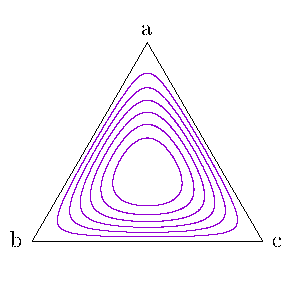
\includegraphics[width=0.7\linewidth]{figures/portrait}
	\caption{Trajectoires macroscopiques dans l'espace des phases du système.}
	\label{fig:portrait}
\end{figure}



\par La dynamique macroscopique possède deux invariants, ce qui le rend intégrable exactement. Le premier est trivial et est donné par la loi de conservation $a+b+c=1$. Le second est le produit $\rho = abc$, en effet
%
\begin{equation}\label{rho_invariant}
\begin{split}
	\frac{\dd \rho}{\dd t} 
	&= \dot a bc + a \dot b c + ab \dot c \\
	&= ka(b-c) + kb(c-a) + kc(a-b) \\
	&= 0
\end{split}
\end{equation}
%

{\color{red} Généralisation d espèces}

{\color{red} Deux hamiltoniens H0 et H1 ??}


\section{Dynamiques micro et mésoscopiques}
\label{section_micro}

\par La dynamique microscopique est un processus de Markov pour lequel un état du système $\{A,B,C\}$ subit les transitions 
%
\begin{equation}\label{dyn_micro}
\begin{split}
	\{A,B,C\} &\longrightarrow \{A+1,B-1,C\}  \qquad \text{fréquence = } k\, AB, \\
	\{A,B,C\} &\longrightarrow \{A,B+1,C-1\}  \qquad \text{fréquence = } k\, BC, \\
	\{A,B,C\} &\longrightarrow \{A-1,B,C+1\}  \qquad \text{fréquence = } k\, CA.
\end{split}
\end{equation}
%
L'équation maîtresse associée est 
%
\begin{equation}\label{eq_maitresse}
\begin{split}
	\frac{\dd}{\dd t}\, P_t(A,B,C) 
	&= k\, (A-1)(B+1)\, P_t(A-1,B+1,C) - k\, AB\, P_t(A,B,C) \\
	{\color{white}\frac{\dd}{\dd t}} % for uniform spacing
	&+ k\, (B-1)(C+1)\, P_t(A,B-1,C+1) - k\, BC\, P_t(A,B,C) \\
	{\color{white}\frac{\dd}{\dd t}} % for uniform spacing
	&+ k\, (C-1)(A+1)\, P_t(A+1,B,C-1) - k\, CA\, P_t(A,B,C).
\end{split}
\end{equation}
% 
Au contraire de la dynamique macroscopique déterministe, l'évolution microscopique ne préserve pas l'invariant $\rho = abc = ABC/N^3$. Le caractère aléatoire des trajectoires microscopiques mène finalement à l'extinction d'une des trois espèces, qui est irréversible. 

\par En développant l'équation maîtresse en puissances de $\epsilon = 1/N$, on déduit l'équation de Fokker-Planck 
%
\begin{equation}\label{eq_FP}
	\partial_t \Psi_t = - \partial_i ( \mu_i \Psi_t ) + \partial_i\partial_j (D_{ij} \Psi_t),
\end{equation}
%
où $\Psi_t(a,b,c)$ est la densité de probabilité pour les fractions $a,b,c$,
%
\begin{equation}\label{lien_psi_proba}
	\Psi_t(a,b,c) = N^3 P_t(A,B,C) = \epsilon^{-3} P_t(a/\epsilon, b/\epsilon, c/\epsilon).
\end{equation}

\par Cette équation décrit la dynamique du système à une échelle intermédiaire, que l'on pourrait qualifier de "mésoscopique". L'équation de Fokker-Planck s'obtient dans la limite de grand $N$, mais nous gardons encore des puissances de $1/N$ dans le terme de diffusion. Cette description garde donc le caractère aléatoire des trajectoires microscopiques. Ce niveau de description est approprié pour étudier des phénomènes d'origine stochastique, comme l'extinction d'une des espèces du modèle, en ayant la possibilité d'employer les outils de calcul différentiel, qui s'appliquent à une description en variables continues. 

\par Il est important de souligner que l'échelle de temps apparaissant dans les équations maîtresse et de Fokker-Planck n'est pas la même. Pour formuler l'équation de Fokker-Planck ainsi, il est nécessaire d'absorber les paramètres $k$ et $N$ dans la variable temporelle (voir section suivante). 

\par Les quantités $\mu_i$ et $D_{ij}$ sont respectivement les vecteurs de dérive et la matrice de diffusion. Le vecteur de dérive est donné par 
%
\begin{equation}\label{mu_i_expr}
	\boldsymbol\mu^T = 
	\begin{bmatrix} a(b-c) & b(c-a) & c(a-b) \end{bmatrix}
\end{equation}
%
et la matrice de diffusion est
%
\begin{equation}\label{D_ij_expr}
	\bold D = \frac{\epsilon}{2}
	\begin{bmatrix}
	a(b+c) & -ab & -ac \\
	-ab & b(c+a) & -bc \\
	-ac & -bc & c(a+b)
	\end{bmatrix}.
\end{equation}
%

\par L'équation différentielle stochastique associée est, selon la convention de Itô,
%
\begin{equation}\label{SDE_abc}
	\dd \bold r_t = \boldsymbol \mu (\bold r_t) \, \dd t + \boldsymbol \sigma(\bold r_t) \, \dd \bold W_t,
\end{equation}
où $\bold r_t = (a,b,c)$, $\bold D = \frac 12 \boldsymbol \sigma \boldsymbol \sigma^T$, et $\bold W_t$ est un processus de Wien de moyenne nulle et de variance unité.

\par À partir de l'équation de Fokker-Planck (eq \ref{eq_FP}), nous pouvons calculer l'évolution de la moyenne de l'invariant déterministe $\rho=abc\geq 0$. On constate que celui-ci ne peut que décroître, menant inéluctablement les trajectoires sur les bords de l'espace des phase, où $\rho=0$. En effet,
%
\begin{equation}\label{dt_rho_initial}
\begin{split}
	\frac{\dd}{\dd t} \langle \rho \rangle 
	&= \frac{\dd}{\dd t} \int abc \, \Psi_t(a,b,c) \, \dd a \, \dd b \, \dd c \\
	&= \int abc \, \partial_t \Psi_t(a,b,c) \, \dd a \, \dd b \, \dd c \\
	&= - \int abc \, \partial_i (\mu_i \, \Psi_t) \, \dd a \, \dd b \, \dd c 
	+ \int abc \, \partial_i\partial_j (D_{ij} \, \Psi_t) \, \dd a \, \dd b \, \dd c \\
	&= \int \partial_i (abc) \, \mu_i \, \Psi_t \, \dd a \, \dd b \, \dd c
	+ \int \partial_i\partial_j (abc) \, D_{ij} \, \Psi_t \, \dd a \, \dd b \, \dd c,
\end{split}
\end{equation}
%
la dernière ligne s'obtenant en intégrant par parties. La première intégrale correspond à l'évolution déterministe, qui doit s'annuler pour retrouver l'invariance de $\rho$. On vérifie bien que 
%
\begin{equation}\label{dt_rho_contrib_det}
	\partial_i(abc) \mu_i = bc\, a(b-c) + ac\, b(c-a) + ab\, c(a-b) = 0.
\end{equation}
%
La deuxième intégrale correspond à l'évolution stochastique, pour laquelle
%
\begin{equation}\label{dt_rho_contrib_stoch}
	\partial_i\partial_j (abc) \, D_{ij} = c(-ab)+b(-ac)+c(-ab)+a(-bc)+b(-ac)+a(-bc) = -6\, abc.
\end{equation}
Ainsi,
%
\begin{equation}\label{dt_rho_final}
	\frac{\dd}{\dd t} \langle \rho \rangle = -6 \int abc \, \Psi_t \, \dd a \, \dd b \, \dd c = -6 \langle \rho \rangle < 0.
\end{equation}
%

\section{Développement de Kramers-Moyal de l'équation maîtresse}
\label{section_kramers_moyal}

\par On commence par exprimer l'équation maîtresse (eq \ref{eq_maitresse}) avec les variables "mésoscopiques" $\Psi_t$, $a,b,c$ et $\epsilon=1/N$. On obtient
%
\begin{equation}\label{eq_maitresse_minuscules}
\begin{split}
	\epsilon ^3 \partial_t \Psi_t(a,b,c) 
	&= k \left( \frac a \epsilon - 1 \right) \left( \frac b \epsilon + 1\right)  \, \epsilon^3 \Psi_t(a-\epsilon, b+\epsilon, c) \\
	&- k\, \frac a \epsilon \frac b \epsilon \, \epsilon^3 \Psi_t(a,b,c) + p.c. \,\, ,
\end{split}
\end{equation}
%
où nous avons symbolisé par $p.c.$ les termes issus de permutations cycliques par rapport à $a,b,c$ dans les termes déjà notés. Cette équation peut être réarrangée en
%
\begin{equation}\label{eq_maitresse_minuscules_clean}
\begin{split}
	\frac{\epsilon^2}{k}\, \partial_t \Psi_t(a,b,c) 
	&= (a-\epsilon)(b+\epsilon)  \, \Psi_t(a-\epsilon, b+\epsilon, c) 
	- ab \, \Psi_t(a,b,c) + p.c. \,\, .
\end{split}
\end{equation}
%

\par On développe ensuite en puissance de $\epsilon$, en ne gardant que les termes d'ordre inférieur ou égal à deux. On commence par développer le produit $(a-\epsilon)(b+\epsilon)$,
%
\begin{equation}\label{moyal_dev_epsilon_produit}
\begin{split}
	\frac{\epsilon^2}{k}\, \partial_t \Psi_t(a,b,c) 
	&= ab \, \Psi_t(a-\epsilon, b+\epsilon, c) + (a-b)\epsilon \, \Psi_t(a-\epsilon, b+\epsilon, c) \\
	&\quad - \epsilon^2 \, \Psi_t(a-\epsilon, b+\epsilon, c) - ab \, \Psi_t(a, b, c) + p.c.
\end{split}
\end{equation}
%
Ensuite, on développe les densités de probabilité en série de Taylor,
%
\begin{equation}\label{moyal_dev_epsilon_taylor}
\begin{split}
	\frac{\epsilon^2}{k}\, \partial_t \Psi_t(a,b,c) 
	&= \cancel{ab \, \Psi_t(a, b, c)} 
	- {\color{purple} ab \, \epsilon \, \partial_a \Psi_t(a,b,c) }
	+ {\color{purple} ab \, \epsilon \, \partial_b \Psi_t(a,b,c) }\\
	{\color{white} \frac{\epsilon^2}{k} } % for uniform spacing
	&\quad + {\color{blue} \frac{\epsilon^2}{2} \, \partial_a^2 \Psi_t(a,b,c) }
	+ {\color{blue} \frac{\epsilon^2}{2} \, \partial_b^2 \Psi_t(a,b,c) }
	+ {\color{blue} \epsilon^2 \, \partial_a \partial_b \Psi_t(a,b,c) }\\
	{\color{white} \frac{\epsilon^2}{k} } % for uniform spacing  
	&\quad + \cancel{\color{brown} (a-b) \,\epsilon \, \Psi_t(a, b, c) }
	- {\color{cyan} (a-b) \,\epsilon^2 \, \partial_a \Psi_t(a,b,c) }\\
	{\color{white} \frac{\epsilon^2}{k} } % for uniform spacing
	&\quad + {\color{cyan} (a-b) \,\epsilon^2 \, \partial_b \Psi_t(a,b,c) } 
	- {\color{green!60!black} \epsilon^2 \, \Psi_t(a, b, c) } 
	- \cancel{ab \, \Psi_t(a, b, c)} \\
	&\quad + p.c.
\end{split}
\end{equation}
%
Remarquons que le terme coloré en brun s'annule avec ses homologues issus des permutations cycliques en $a,b,c$. 

\par La dernière étape consiste à redéfinir l'échelle de temps en absorbant $\epsilon$ et $k$ dans $t$, de sorte que 
%
\begin{equation}\label{moyal_redef_temps}
	\frac{k}{\epsilon} \, t \rightarrow t,
\end{equation}
%
nous obtenons ainsi 
%
\begin{equation}\label{moyal_dev_epsilon_complet}
\begin{split}
	\partial_t \Psi_t(a,b,c) 
	&= {\color{purple} ab \, \partial_a \Psi_t(a,b,c) }
	+ {\color{purple} ab \, \partial_b \Psi_t(a,b,c) }\\
	&\quad + {\color{blue} \frac{\epsilon}{2} \, \partial_a^2 \Psi_t(a,b,c) }
	+ {\color{blue} \frac{\epsilon}{2} \, \partial_b^2 \Psi_t(a,b,c) }
	+ {\color{blue} \epsilon \, \partial_a \partial_b \Psi_t(a,b,c) }\\
	&\quad - {\color{cyan} (a-b) \,\epsilon \, \partial_a \Psi_t(a,b,c) }
	+ {\color{cyan} (a-b) \,\epsilon \, \partial_b \Psi_t(a,b,c) } \\
	&\quad- {\color{green!60!black} \epsilon \, \Psi_t(a, b, c) } 
	+ p.c.
\end{split}
\end{equation}
%

\par Pour voir que ce développement mène à l'équation de Fokker-Planck (eq \ref{eq_FP}), il est plus facile de partir de cette dernière équation et développer les expressions de $\mu_i$ et $D_{ij}$. Cela donne
%
\begin{equation}\label{moyal_dev_eq_FP}
\begin{split}
	\partial_t \Psi_t
	&= - \partial_i \mu_i \, \Psi_t
	- {\color{purple} \mu_i \, \partial_i \Psi_t }
	+ {\color{green!60!black} \partial_i\partial_j D_{ij} \, \Psi_t }
	+ {\color{cyan} 2 \partial_i D_{ij} \, \partial_j \Psi_t }
	+ {\color{blue} D_{ij} \,  \partial_i\partial_j \Psi_t } \\
	&= - \cancel{(b-c) \, \Psi_t} - \cancel{p.c.}
	%- \cancel{(c-a) \, \Psi_t}
	%- \cancel{(a-b) \, \Psi_t} \\
	- {\color{purple} a(b-c)\, \partial_a \Psi_t }
	- {\color{purple} p.c. }
	%- {\color{purple} b(c-a)\, \partial_b \Psi_t }
	%- {\color{purple} c(a-b)\, \partial_c \Psi_t } \\
	+ {\color{green!60!black} \frac \epsilon 2 \, [0-\Psi_t-\Psi_t] }
	+ {\color{green!60!black} p.c. } \\
	&\quad + {\color{cyan} \epsilon \, [ (b+c) \, \partial_a \Psi_t - b \, \partial_b \Psi_t - c \, \partial_c \Psi_t ] }
	+ {\color{cyan} p.c. } \\
	&\quad + {\color{blue} \frac \epsilon 2 \, [ a(b+c) \, \partial_a^2 \Psi_t - ab \, \partial_a\partial_b \Psi_t - ac \, \partial_a\partial_c \Psi_t ] }
	+ {\color{blue} p.c. }
\end{split} 
\end{equation}
%
La correspondance entre les termes violets, vert et bleus des équations \ref{moyal_redef_temps} et \ref{moyal_dev_eq_FP} est assez facile à voir, en tenant compte des permutations cycliques. Pour les termes cyan, il faut employer la relation de conservation $a+b+c=1$. Par example, les termes en $\partial_a\Psi_t$ dans l'équation \ref{moyal_dev_eq_FP} peuvent être écrits comme
%
\begin{equation}\label{moyal_terme_cyan_corresp}
	\epsilon\, (b+c)\, \partial_a\Psi_t -2\epsilon\, a\, \partial_a\Psi_t = \epsilon\, (b-a)\, \partial_a\Psi_t + \epsilon\, (c-a)\, \partial_a\Psi_t.
\end{equation}
%

\section{Réduction à un processus radial}
\label{section_stoch_averaging}

\par L'évolution dictée par l'équation de Fokker-Planck montre que la dérive le long du vecteur $\boldsymbol \mu$, se produit sur des temps beaucoup plus courts que le phénomène de diffusion. Le rapport entre les deux échelles est donné par le facteur $\epsilon = 1/N$ dans la matrice de diffusion (eq \ref{D_ij_expr}), qui montre que la diffusion est de moins en moins importante dans la limite $N\rightarrow\infty$. Cette différence d'échelle implique qu'une densité de probabilité piquée autour d'un point de l'espace des phase va évoluer le long d'une orbite déterministe beaucoup plus vite qu'elle ne va s'étaler sur les orbites voisines.

\par Une conséquence importante est que nous pouvons approximer l'évolution de l'invariant $\rho$ comme un processus stochastique unidimensionnel. %L'idée est de "moyenner" le terme diffusif le long des trajectoires déterministes. 
Cette simplification nous intéresse tout particulièrement car les outils que nous allons utiliser pour traiter les extinctions dans le système s'appliquent beaucoup plus simplement aux processus unidimensionnels.

\par On commence par exprimer les accroissements $\dd \rho$ en termes de $\dd \bold r$,
%
\begin{equation}\label{averaging_drho_1}
	\dd\rho = \rho(\bold r+ \dd \bold r) - \rho (\bold r) = \partial_i\rho \, \dd r_i + \frac 12 \partial_i \partial_j \rho \, \dd r_i \, \dd r_j.
\end{equation}
% 
Ensuite, nous substituons l'équation différentielle stochastique pour $\bold r$ (eq \ref{SDE_abc}),
%
\begin{equation}\label{averaging_drho_2}
	\dd \rho = \mu_i\partial_i\rho \, \dd t + \sigma_{ij} \, \partial_i\rho \, \dd W_j + \frac 12 \, \partial_i \partial_j \rho \  \sigma_{ik}\sigma_{jl} \, \dd W_k \, \dd W_l.
\end{equation}
%
La relation \ref{dt_rho_contrib_det} montre que le premier terme s'annule. Nous transformons le dernier terme en utilisant les relations $\dd W_k \, \dd W_l = \delta_{kl} \, \dd t$ et $\frac 12 \boldsymbol \sigma \boldsymbol \sigma^T = \bold D$ pour obtenir
%
\begin{equation}\label{averaging_drho_3}
	\dd \rho = \partial_i \partial_j \rho \ D_{ij} \, \dd t + \sigma_{ij} \, \partial_i\rho \, \dd W_j.
\end{equation}
%
\par Le premier terme est un terme de dérive pour l'évolution de $\rho$, mais provient de la diffusion dans l'évolution des variables $a,b,c$. Il s'évalue à
%
\begin{equation}\label{drho_derive_stoch}
\begin{split}
	\partial_i \partial_j \rho \ D_{ij}
	&= \frac \epsilon 2 \, [ a(b+c) \, \cancel{ \partial_a^2(abc)} + (-ab) \, \partial_a \partial_b(abc) + (-ac) \, \partial_a\partial_c(abc) \\
	&\qquad + (-ab) \, \partial_b \partial_a (abc) + b(c+a) \, \cancel{ \partial_b^2(abc)} + (-bc) \, \partial_b\partial_c(abc) \\
	&\qquad + (-ac) \, \partial_c\partial_a(abc) + (-bc) \, \partial_c\partial_b(abc) + c(a+b) \, \cancel{ \partial_c^2(abc)} \,] \\
	&= \frac \epsilon 2 \, [-6 \, abc \,] = -3\epsilon \, \rho = -\frac 3N \, \rho.
\end{split}
\end{equation}
%
Le deuxième terme cache une dépendance en $N$ à l'intérieur de $\sigma_{ij}$. Pour se rapprocher de la convention employée dans \cite{frey2012}, nous utilisons les matrices $\bold C$ et $\bold B$, indépendentes de $N$, telles que $\boldsymbol \sigma = \frac{1}{\sqrt{N}} \bold C$ et $\bold D = \frac{1}{2N} \bold B$, et $\bold B = \bold C \bold C^T$, pour réécrire notre équation différentielle stochastique sous la forme
%
\begin{equation}\label{averaging_drho_4}
	\dd \rho = -\frac 3N \, \rho \, \dd t + \frac{1}{\sqrt{N}}\, C_{ij} \, \partial_i\rho \, \dd W_j.
\end{equation}
%

\par À ce stade, notre équation pour $\dd \rho$ contient encore des références à la dynamique dans l'espace des phases $a,b,c$ de part la dimension du bruit $\dd W_j$ et à travers $C_{ij}$ qui dépend encore explicitement de $a,b,c$. Frey et al. éliminent ces problèmes en moyennant le terme de diffusion sur les trajectoires du système déterministe \cite{frey2012}. Ils invoquent un théorème de Khasminskii \cite{khasminskij1968} pour obtenir un processus unidimensionnel
%
\begin{equation}\label{averaging_drho_final}
	\dd \rho = -\frac 3N \,\rho\,\dd t + \frac{1}{\sqrt{N}} \sqrt{\bar D(\rho)} \,\dd W
\end{equation}
%  
avec un coefficient de diffusion effectif obtenu en moyennant un coefficient de diffusion $D(a,b,c)$, local sur la trajectoire, sur une période complète de l'orbite,
%
\begin{equation}\label{D_rho_from_D_abc}
	\bar D(\rho) = \frac{1}{T(\rho)} \int_0^{T(\rho)} D(a,b,c) \ \dd t.
\end{equation}
%
Ils fournissent la formule
%
\begin{equation}\label{formule_D_abc}
	D(a,b,c) = (\bold C \bold \nabla\rho)^T(\bold C \bold \nabla\rho) = (\bold \nabla\rho)^T \bold B \, (\bold \nabla\rho),
\end{equation}
%
ce qui nous permet d'évaluer $D(a,b,c)$,
%
\begin{equation}\label{eval_D_abc}
\begin{split}
	D(a,b,c) 
	&= \partial_a(abc) \, a(b+c) \, \partial_a(abc) 
	+ \partial_a(abc) \, (-ab) \, \partial_b(abc) \\
	&\quad + \partial_a(abc) \, (-ac) \, \partial_c(abc) + p.c. \\
%	&\quad + \partial_b(abc) \, (-ab) \, \partial_a(abc)
%	+ \partial_b(abc) \, b(c+a) \, \partial_b(abc)
%	+ \partial_b(abc) \, (-bc) \, \partial_c(abc) \\
%	&\quad + \partial_c(abc) \, (-ac) \, \partial_a(abc)
%	+ \partial_c(abc) \, (-bc) \, \partial_b(abc)
%	+ \partial_c(abc) \, c(a+b) \, \partial_c(abc) \\
	&= a(b+c) \, b^2c^2 - a^2b^2c^2 - a^2b^2c^2 + p.c. \\
	&= (abc)^2 \left( \frac{b+c}{a}-2 \right)  + p.c. \\ 
	&= \rho^2 \left( \frac{1-a}{a}-2 \right)  + p.c. \\
	&= \rho^2 \left( \frac{1}{a}-3 \right)  + p.c. \\
	&= \rho^2 \left( -9 + \frac 1a + \frac 1b + \frac 1c \right) 
\end{split}
\end{equation}
%


\subsection*{Justifications de l'étape de moyennage stochastique}

\par Dans l'article de Frey et al. \cite{frey2012}, peu d'explications sont fournies concernant l'étape de moyennage. Il m'a été difficile de trouver des références dans la littérature détaillant cette procédure. J'identifie deux points qui ne sont pas clairs. Le premier est le passage d'un processus de Wien tridimensionnel à un processus unidimensionnel. Le second est l'étape de moyennage elle-même, c'est à dire la formule {\color{red}reference}. Pourquoi la moyenne se fait sur la grandeur $D$ et pas une autre, par example sa racine?

\par Concernant le premier point, il semble possible de réduire la dimension du processus de Wien $\dd W_j$ en remarquant que la matrice $\bold C$ est définie à une multiplication près $\bold C \bold S$, à condition que la matrice $\bold S$ soit orthogonale. Ceci est dû au fait que cette transformation ne modifie pas la matrice de diffusion 
%
\begin{equation}\label{invariance_B}
	\bold B' = (\bold C \bold S) (\bold C \bold S)^T = \bold C \, \bold S \bold S^T \bold C^T = \bold C \bold C^T = \bold B.
\end{equation}
%
Cette propriété traduit le fait que le terme de diffusion de l'équation différentielle stochastique peut être construite avec un bruit $\dd W_j$ donné dans une base quelconque, sans changer la nature du processus qui en résulte. %La conséquence qui nous intéresse est que l'on peut formuler notre équation dans une base pour laquelle l'un des axes est aligné avec le gradient de $\rho$. Ainsi, {\color{red} CONTINUER}
La conséquence qui nous intéresse est que l'on peut toujours transormer $\bold C$ en une matrice triangulaire (cf. décomposition QR). Dans une base pour laquelle l'un des axes est aligné avec le gradient de $\rho$, nous avons $\partial_2\rho = \partial_3\rho = 0$ et ainsi
%
\begin{equation}\label{reduction_dW_1D_1}
	C_{ij} \, \partial_i\rho \, \dd W_j = 
	C_{1j} \, \partial_1\rho \, \dd W_j + 
	\cancel{ C_{2j} \, \partial_2\rho \, \dd W_j } + 
	\cancel{ C_{3j} \, \partial_3\rho \, \dd W_j }
	= C_{1j} \, \partial_1\rho \, \dd W_j
\end{equation}
%
Comme nous pouvons considérer la matrice $\bold C$ comme étant triangulaire supérieure sans perte de généralité, $C_{12} = C_{13} = 0$ et cela réduit donc la dimension du processus de Wien nécessaire dans l'équation différentielle stochastique,
%
\begin{equation}\label{reduction_dW_1D_2}
	C_{ij} \, \partial_i\rho \, \dd W_j = C_{11} \, \partial_1\rho \, \dd W_1.
\end{equation}
%
Nous pouvons donc réécrire l'équation \ref{averaging_drho_4} avec un processus de Wien unidimensionnel,
%
\begin{equation}\label{averaging_drho_5}
\dd \rho = -\frac 3N \, \rho \, \dd t + \frac{1}{\sqrt{N}}\, \sqrt{D} \, \partial_i\rho \, \dd W,
\end{equation}
%
en utilisant un coefficient de diffusion $D(a,b,c)$ qui préserve la variance du processus,
%
\begin{equation}\label{expr_D_abc_variance}
	D(a,b,c) = (\bold C \bold \nabla\rho)^T(\bold C \bold \nabla\rho) = (\bold \nabla\rho)^T \bold B \, (\bold \nabla\rho).
\end{equation}
%

\section{Problème de première sortie d'un intervalle}
\label{section_echap}

\par Le problème de calculer le temps moyen d'extinction d'une espèce dans le modèle de prédation cyclique est équivalent à calculer le temps moyen de première sortie de la région ${a,b,c|a,b,c>0}$, où chaque espèce est présente avec une fraction non nulle. Une fois que la diffusion dans le système est réduite à un processus radial, le problème est unidimensionnel et la région à échapper est un simple intervalle, de frontières $\rho=0$ et $\rho=1/27$. Pour calculer le temps moyen d'extinction, nous allons nous baser sur ce parallèle entre les deux problèmes et utiliser les techniques d'analyse servant à résoudre le problème de première sortie pour un processus stochastique homogène 1D.

\par On suppose que le processus 1D est régi par l'équation de Fokker-Planck
%
\begin{equation}\label{echap_eq_FP}
	\partial_t p_t(x) = - \partial_x[ A(x) \, p_t(x) ] + \frac 12 \, \partial_x^2 [ B(x) \, p_t(x) ] .
\end{equation}
%
Notre intervalle à échapper est $[a,b]$ avec une barrière absorbante en $a$ et répulsive en $b$. Nous commençons par nous intéresser à la quantité 
%
\begin{equation}\label{echap_def_G}
	G(x,t) = \int_a^b \dd y \, p(y,t|x,0),
\end{equation}
%
qui est la probabilité d'être encore dans l'intervalle au temps $t$, sachant que l'on démarre en $x$.

\par Étant donné que l'équation de Fokker-Planck est homogène en le temps, nous avons que 
%
\begin{equation}\label{echap_homogeneite_p}
	p(y,t|x,0) = p(y,0|x,-t)
\end{equation}
%
et nous pouvons ainsi formuler l'équation de Fokker-Planck réverse en substituant la probabilité conditionelle dans l'équation originale {\color{red} clarifier?} 
%
\begin{equation}\label{echap_eq_FP_backward}
	\partial_t p_t(y,t|x,0) = -A(x)\, \partial_x p_t(y,t|x,0) + \frac 12 \, B(x)\, \partial_x^2 p_t(y,t|x,0).
\end{equation}
%
À la différence de l'équation de Fokker-Planck directe, l'équation réverse voit les dérivées agir directement sur la densité de probabilité. Cela nous permet de formuler une équation différentielle pour une observable, comme $G(x,t)$. En intégrant sur $y$, l'intégrale passe sous les dérivées en $x$,
%
\begin{equation}\label{echao_int_FP_backward}
	\partial_t \int_a^b \dd y \, p(y,t|x,0) = - A(x) \, \partial_x \int_a^b \dd y \, p(y,t|x,0) + \frac 12 \, B(x) \, \partial_x^2 \int_a^b \dd y \, p(y,t|x,0),
\end{equation}
%
et nous obtenons une équation différentielle pour $G(x,t)$,
%
\begin{equation}\label{echap_eq_G}
	\partial_t G(x,t) = - A(x) \, \partial_x G(x,t) + \frac 12 \, B(x) \, \partial_x^2 G(x,t).
\end{equation}
%

\par Le temps moyen de première sortie est une fonction de la position de départ dans l'intervalle. Il est donné par {\color{red} clarifier?}
%
\begin{equation}\label{echap_expr_Tx}
	T(x) = - \int_0^\infty t \, \partial_t G(x,t) \, \dd t \, = \int_0^\infty  G(x,t) \, \dd t \, .
\end{equation}
%
En intégrant l'équation pour $G(x,t)$ par rapport au temps,
%
\begin{equation}\label{echap_int_eq_G_1}
	 - \int_0^\infty A(x) \, \partial_x G(x,t) \, \dd t + \frac 12 \int_0^\infty \, B(x) \, \partial_x^2 G(x,t) \, \dd t = \int_0^\infty \partial_t G(x,t) \, \dd t \, ,
\end{equation}
%
\begin{equation}\label{echap_int_eq_G_2}
	- A(x) \, \partial_x \int_0^\infty G(x,t) \, \dd t + \frac 12 \, B(x) \, \partial_x^2 \int_0^\infty G(x,t) \, \dd t = G(x,\infty) - G(x,0) \, ,
\end{equation}
%
on obtient une équation différentielle pour $T(x)$,
%
\begin{equation}\label{echap_eq_T}
	-A(x) \, \partial_x T(x) + \frac 12 \, B(x) \, \partial_x^2 T(x) = -1.
\end{equation}
%
Le membre de droite de l'équation \ref{echap_int_eq_G_2} s'évalue à $-1$ car au temps initial la particule est dans l'intervalle avec probabilité $1$ et donc $G(x,0)=1$. De même, dans la limite de temps infini, la particule fini tôt ou tard par être absorbée par la barrière $a$, ainsi $G(x,\infty)=0$. 

\par Pour résoudre l'équation différentielle \ref{echap_eq_T}, il reste à spécifier les conditions aux bords. La barrière $a$ est absorbante, une particule se trouvant en $x=a$ est ainsi immédiatement retirée de l'intervalle $[a,b]$ nous avons donc $G(a,0)=0$ comme condition à ce bord. Sur le temps de sortie, cette condition se traduit par $T(a)=0$. La barrière $b$ est répulsive, cela signifie que le flux net de probabilité est nul en $b$, et donc $\partial_x G(b,0) = 0$. Cela se traduit par $\partial_x T(b) = 0$.

\par La résolution de l'équation différentielle pour $T(x)$ peut se faire par intégration directe. En posant $Y(x) = \partial_x T(x)$, l'équation \ref{echap_eq_T} devient 
%
\begin{equation}\label{echap_eq_T_int_directe}
	\partial_x Y(x) - \frac{2A(x)}{B(x)} Y(x) = -\frac{2}{B(x)}.
\end{equation}
%
La solution
\footnote{
	Pour résoudre une équation différentielle du type $f'(x)+p(x)f(x)=q(x)$, on peut chercher à l'écrire sous la forme directement intégrable $M'(x) = N(x)$. Pour cela, on multiplie les deux côtés de l'équation par $\exp(\int p)$. Le terme de droite s'écrit alors explicitement comme la dérivée d'un produit, $M' = f'\exp(\int p) + f p \exp(\int p)$, avec $M = f\exp(\int p)$. Le terme de gauche est $N = q \exp(\int p)$. Nous pouvons ensuite intégrer directement pour obtenir $M = \int N + c_0$ et donc $f = \exp(-\int p) \int N + c_0 \exp(-\int p)$.
}
pour $Y(x)$ est 
%
\begin{equation}\label{echap_sol_Y_avec_c0}
\begin{split}
	Y(x) &= \exp\left[ - \int_a^x \frac{2 A(y)}{B(y)} \dd y \right]
	\int_a^x \frac{(-2)}{B(y)} \exp\left[ \int_a^y \frac{2 A(z)}{B(z)} \dd z\right] \dd y \\
	&\quad + c_0 \exp\left[ - \int_a^x \frac{2 A(y)}{B(y)} \dd y \right].
\end{split}	
\end{equation}
%
La condition au bord $Y(b)=\partial_x T(b)=0$ impose que 
%
\begin{equation}\label{echap_sol_Y_bord_b}
	c_0 = \int_a^x \frac{2}{B(y)} \exp\left[ \int_a^y \frac{2 A(z)}{B(z)} \dd z\right] \dd y,
\end{equation}
%
et donc
%
\begin{equation}\label{echap_sol_Y_sans_c0}
	Y(x) = \exp\left[ - \int_a^x \frac{2 A(y)}{B(y)} \dd y \right]
	\int_x^b \frac{2}{B(y)} \exp\left[ \int_a^y \frac{2 A(z)}{B(z)} \dd z\right] \dd y.
\end{equation}
%
Cette solution donne un temps moyen de première sortie
%
\begin{equation}\label{echap_sol_T_avec_c1}
	T(x) = \int_a^x Y(y) \, \dd y + c_1.
\end{equation}
%
Il est facile de voir que la condition au bord $a$ demande que $c_1=0$. En introduisant la fonction   
%
\begin{equation}\label{echap_psi_x}
	\psi(x) = \exp\left[ \int_a^x \frac{2A(y)}{B(y)} \dd y \right] ,
\end{equation}
%
nous pouvons écrire la solution pour $T(x)$ sous la forme plus lisible
%
\begin{equation}\label{echap_sol_T_finale}
	T(x) = \int_a^x \frac{1}{\psi(y)} \int_y^b \frac{2\psi(z)}{B(z)} \, \dd z \, \dd y.
\end{equation}
%

\par Nous avons ainsi obtenu la formule donnant le temps de sortie moyen d'un intervalle pour un processus stochastique unidimensionnel. Cette formule nous permet de calculer le temps moyen d'extinction dans notre modèle de prédation cyclique. De l'équation de Fokker-Planck, nous pouvons identifier les coefficients de dérive et de diffusion
%
\begin{equation}\label{coefs_A_B_radial}
A(\rho) = - \frac 3N \, \rho \qquad \text{et} \qquad 
B(\rho) = \frac 1N \bar D(\rho).
\end{equation}
%
Les bornes $a$ et $b$ sont dans ce cas $\rho=0$ et $\rho=1/27$, respectivement.


\section{Calcul numérique du temps moyen d'extinction}
\label{section_textc_numerique}

\begin{figure}
	\centering
	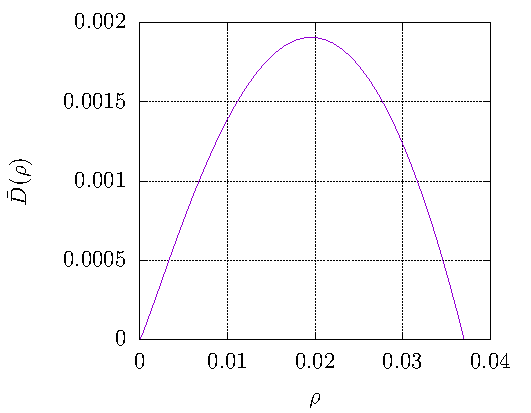
\includegraphics[width=0.7\linewidth]{figures/D_rho}
	\caption{Coefficient de diffusion effectif $\bar D(\rho)$ en fonction de $\rho$.}
	\label{fig:D_rho}
\end{figure}

\par On obtient le temps moyen d'extinction à partir de la formule \ref{echap_sol_T_finale} en calculant les intégrales numériquement. Nous utilisons la méthode des trapèzes pour calculer les intégrales avec une précision quadratique en la discrétisation.

\par La quantité $\bar D(\rho)$ intervenant dans le coefficient de diffusion est aussi calculée numériquement. On utilise l'expression \ref{D_rho_from_D_abc} pour évaluer $\bar D(\rho)$ en sommant $D(a,b,c)$ le long des trajectoires déterministes. Les trajectoires sont générées par l'algorithme d'Euler, qui est amplement suffisant pour cette tâche. Nous partons du point de l'orbite où la fraction de l'espèce $a$ est maximale et intégrons les équations de la dynamique sur une demi-période seulement, étant donné la symétrie de $D(a,b,c)$ sous l'échange $b\leftrightarrow c$ (voir eq \ref{eval_D_abc}).

\par Pour calculer le point d'une orbite $\rho = abc$ qui maximise $a$, il faut remarquer que quand $a$ est maximal nous avons $b=c$. L'état est donc caractérisé par les équations 
%
\begin{equation}\label{syst_a_max}
	\rho = abc = ab^2  \qquad \text{et} \qquad 1 = a+b+c = a+2b
\end{equation}
%
en isolant $a$ on obtient une équation cubique 
%
\begin{equation}\label{eq_a_max}
	\rho = \frac 14 a (1-a)^2.
\end{equation}
%
Bien que les équations polynomiales soient exactement solubles et plutôt que d'utiliser un algorithme de résolution de polynômes, nous procédons simplement de manière itérative pour recherche la solution de cette équation. En partant de $a=1$, nous diminuons la valeur de $a$ par petit à petit jusqu'à ce que les deux membres de l'équation s'équilibrent. Lorsque le point d'équilibre est passé, nous rebroussons chemin et augmentons maintenant $a$ par pas deux fois plus petits que précédemment. Nous répétons cette procédure jusqu'à ce que le pas soit suffisamment petit.

\par Notons que la procédure complète pour calculer le temps d'extinction moyen requiert quatres intégrations: trois pour résoudre le problème d'échappement (voir equations \ref{echap_sol_T_finale} et \ref{echap_psi_x}) et une pour calculer $\bar D(\rho)$. Pour accélérer le calcul, nous calculons $\bar D(\rho)$ à l'avance en plusieurs points de l'intervalle $[0,1/27]$. Ensuite, nous calculons $\bar D(\rho)$ en interpolant les valeurs que nous avions enregistrées. Nous interpolons avec une parabole en utilisant les trois points les plus proches de la valeur désirée. Le calcul peut ainsi être effectué en quelques minutes.

\par Au lieu de calculer le temps d'extinction moyen à partir de la valeur exacte de $\bar D(\rho)$, nous pouvons équalement faire une approximation de bruit constant en utilisant un terme de diffusion constant. Le choix $D=0.001$ fait par Frey et al. \cite{frey2012} donne une assez bonne approximation du résultat exact. La figure {\color{red} figure} montre les courbes obtenues par interpolation et approximation de $\bar D(\rho)$ côte à côte. Cette figure reporte également des résultats de simulations du système, dont nous parlons dans la section suivante. L'accord entre les calculs théorique (interpolation) et les simulation est excellent. Cela montre la qualité de l'approximation de moyennage effectué dans la section \ref{section_stoch_averaging} pour réduire le processus à une dimension.

{\color{red} Comment évolue la qualité de l'approx avec le nombre d'individus $N$?}

%\begin{figure}
%	\centering
%	\begin{subfigure}{.5\textwidth}
%		\centering
%		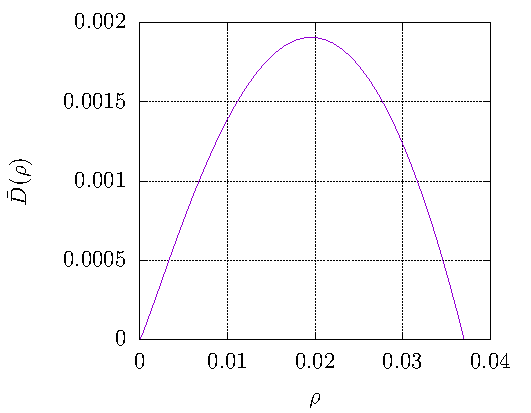
\includegraphics[width=\linewidth]{figures/D_rho}
%	\end{subfigure}%
%	\begin{subfigure}{.5\textwidth}
%		\centering
%		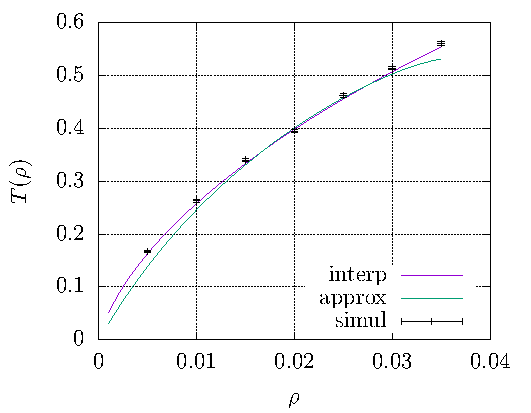
\includegraphics[width=\linewidth]{figures/extc_time_comparison}
%	\end{subfigure}%
%	\caption{Le graphique de gauche représente la fonction $\bar D(\rho)$ donnant l'intensité de la diffusion dans le processus radial. Le graphique de droite donne le temps d'extinction $t/N$ en fonction de la valeur de $\rho$ au point de départ dans le système. La comparaison est faite des temps d'extinction calculé selon l'expression exacte de $\bar D(\rho)$ ("interp"), une approximation à bruit constant $\bar D(\rho)=0.001$ ("approx") ou encore en faisant des simulations du système ("simul"). Dans ces calculs, le nombre d'individus est $N=1000$. Les résultats des simulations sont moyennés sur $10^4$ réalisations. {\color{red} Séparer les figures, agrandir la figure avec les extinctions}}
%	\label{fig:D_rho_et_extc}
%\end{figure}

\begin{figure}[t]
	\centering
	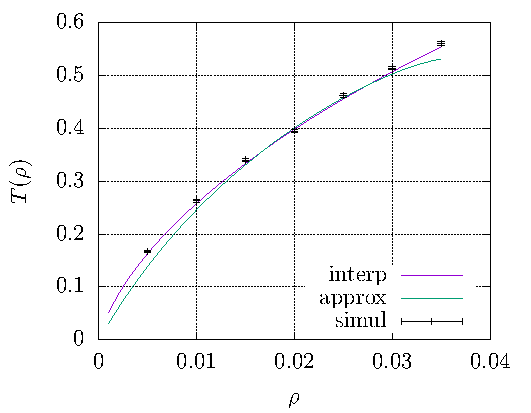
\includegraphics[width=0.9\linewidth]{figures/extc_time_comparison}
	\caption{Temps d'extinction $t/N$ en fonction de la valeur de $\rho$ au point de départ dans le système. La comparaison est faite des temps d'extinction calculé selon l'expression exacte de $\bar D(\rho)$ ("interp"), une approximation à bruit constant $\bar D(\rho)=0.001$ ("approx") ou encore en faisant des simulations du système ("simul"). Dans ces calculs, le nombre d'individus est $N=1000$. Les résultats des simulations sont moyennés sur $10^4$ réalisations.}
	\label{fig:T_extc}
\end{figure}


\section{Simulation du système}
\label{section_simulation}

\par On réalise des simulations numériques du modèle de prédation cyclique en utilisant l'algorithme de Gillespie. Dans cet algorithme, les taux de réactions sont calculés, e.g. $f_{ab} = k AB$, et sommés pour avoir la fréquence à laquelle une réaction quelconque se produit $f_0 = \sum_i\sum_j f_{ij}$. Les réactions sont supposées se produire indépendemment les unes des autres et le temps d'attente avant une réaction suit donc une distribution exponentielle. Ainsi, à chaque réaction effectuée, le temps du système est incrémenté selon
%
\begin{equation}\label{gillespie_incr_temps}
	t \rightarrow t - \frac{1}{f_0} \ln(r),
\end{equation}
%
où $r$ est un nombre aléatoire uniformément distribué entre $0$ et $1$.
La réaction à effectuer est choisie avec un poids de probabilité donné par le rapport entre le taux pour cette réaction et le taux total, $f_{ij}/f_0$.

\par La condition initiale du système est calculée à partir de l'invariant macroscopique $\rho=abc$, entré comme paramètre de la simulation. Nous démarrons la simulation au point de l'orbite où $a$ est maximal, comme expliqué dans la section précédente, les fractions $a,b,c$ calculées sont bien sûr converties en nombres $A,B,C$ d'individus pour chaque espèce. Nous laissons ensuite la simulation tourner jusqu'à ce que l'on détecte une extinction. Plus précisément, nous testons lors de chaque réaction si la population d'une des espèces est tombée à zéro.

\par A la fin de chaque simulation, nous enregistrons le temps d'extinction observé. Les simulations sont répétées un grand nombre de fois, ici $10^4$ réalisations, afin de calculer le temps d'extinction moyen avec une marge d'erreur raisonablement petite. L'erreur reportée pour la détermination de la moyenne est de un écart-type. L'écart-type sur une moyenne de $M$ réalisations est donnée par l'écart-type d'une réalisation divisé par la racine carrée de $M$:
%
\begin{equation}\label{gillespie_err_moyenne}
	\sigma_M = \frac{\sigma}{\sqrt{M}}.
\end{equation}
%


		
\printbibliography

\end{document} 

